% !TeX program = xelatex
% 全国大学生数学建模竞赛论文结构模板
% 说明：本模板只保留优秀论文中高频出现的行文框架，不预置具体建模内容。
% 建议在 Overleaf 中选择 XeLaTeX 编译器。

\documentclass[withoutpreface,bwprint]{cumcmthesis}

% -------------------- 标准竞赛排版 --------------------
\usepackage{cumcm2026}
\usepackage{amsmath,amssymb,bm}
\usepackage{graphicx}
\usepackage{booktabs}
\usepackage{array}
\usepackage{float}
\usepackage{enumitem}
\usepackage{hyperref}
\hypersetup{hidelinks}

% -------------------- 基础版式 --------------------
\setlength{\parindent}{2em}
\setlength{\parskip}{0pt}

% 若需要统一图表文件夹，可直接使用 figures/ 下的文件
\graphicspath{{figures/}}

\begin{document}

% 国赛电子版论文不设置目录，第一页直接从摘要开始。
% ============================================================
% 摘要专用页
% ============================================================
\begin{center}
    {\zihao{3}\bfseries 【论文题目】}
\end{center}

\vspace{0.8em}

\noindent\textbf{摘要：}
【在此填写摘要。结构通常为：总体思路 + 各问题所建模型/方法 + 核心结果 + 必要的模型评价。】

\vspace{0.8em}

\noindent\textbf{关键词：}
【关键词1；关键词2；关键词3；关键词4】

\newpage

% ============================================================
% 一、问题重述
% ============================================================
\section{问题重述}

\subsection{问题背景}
% 只重述研究背景、对象和任务场景，不提前展开模型细节。

\subsection{题目信息与关键条件}
% 若题面信息较少，可删去本小节并并入“问题提出”。

\subsection{问题提出}
% 按问题一、问题二、……依次压缩重述各子任务。

% ============================================================
% 二、问题分析
% ============================================================
\section{问题分析}

\subsection{问题一的分析}

\subsection{问题二的分析}

\subsection{问题三的分析}

\subsection{问题四的分析}

% 若赛题有第五问，可取消下一行注释：
% \subsection{问题五的分析}

\subsection{总体建模思路与模型概述}
% 可放总体流程图、各问题之间的承接关系。
% 若篇幅紧张，也可删除本小节，将总体思路融入前四小节。

% ============================================================
% 三、模型假设
% ============================================================
\section{模型假设}

\begin{enumerate}[label=\arabic*.]
    \item 【假设1】
    \item 【假设2】
    \item 【假设3】
\end{enumerate}

% ============================================================
% 四、符号说明
% ============================================================
\section{符号说明}

% 建议使用三线表，只列正文中反复使用的核心符号。
\begin{table}[H]
    \centering
    \caption{主要符号说明}
    \begin{tabular}{ccc}
        \toprule
        符号 & 含义 & 单位 \\
        \midrule
        $\cdots$ & 【含义】 & 【单位】 \\
        \bottomrule
    \end{tabular}
\end{table}

% ============================================================
% 五、数据预处理（数据型赛题建议保留；纯机理题可整节删除）
% ============================================================
\section{数据预处理与基础分析}

\subsection{数据清洗与整理}

\subsection{数据特征与统计描述}

\subsection{关键参数的计算或标定}
% 若不存在参数标定，可删除本小节。

% ============================================================
% 六、模型的建立与求解
% 高频主线：模型建立 -> 求解方法 -> 结果分析 -> 检验/敏感性
% ============================================================
\section{模型的建立与求解}

\subsection{问题一模型的建立与求解}
\subsubsection{模型准备与变量定义}
\subsubsection{模型建立}
\subsubsection{求解方法与算法流程}
\subsubsection{结果与分析}
\subsubsection{模型检验或敏感性分析}
% 若本问无需单独检验，可删除上一小节。

\subsection{问题二模型的建立与求解}
\subsubsection{模型准备与问题一模型的承接}
\subsubsection{模型建立或修正}
\subsubsection{求解方法与算法流程}
\subsubsection{结果与分析}
\subsubsection{模型检验或敏感性分析}

\subsection{问题三模型的建立与求解}
\subsubsection{模型准备与前述模型的承接}
\subsubsection{模型建立或修正}
\subsubsection{求解方法与算法流程}
\subsubsection{结果与分析}
\subsubsection{对比分析或模型检验}

\subsection{问题四模型的建立与求解}
\subsubsection{模型准备与前述模型的承接}
\subsubsection{模型建立或扩展}
\subsubsection{求解方法与算法流程}
\subsubsection{结果与分析}
\subsubsection{模型检验或讨论}

% 若赛题有第五问，可复制以下结构：
% \subsection{问题五模型的建立与求解}
% \subsubsection{模型建立}
% \subsubsection{求解方法与算法流程}
% \subsubsection{结果与分析}

\subsection{公式、图表与交叉引用示例}
\begin{equation}
 E = mc^2
 \label{eq:placeholder-energy}
\end{equation}
式\eqref{eq:placeholder-energy}为带编号公式。
\begin{figure}[htbp]
\centering
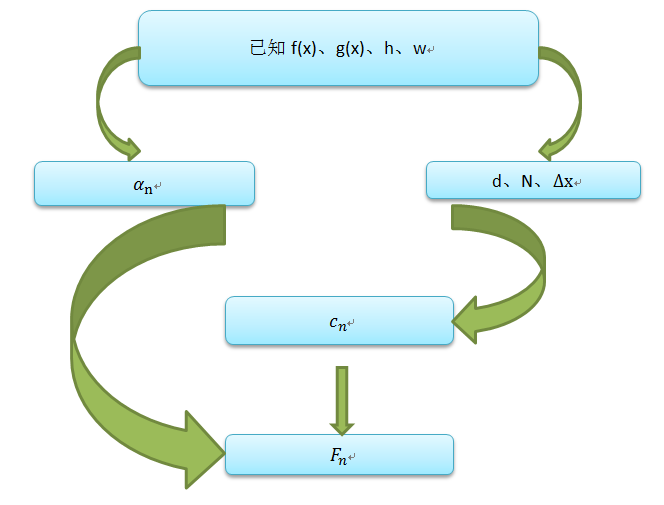
\includegraphics[width=0.55\textwidth]{example_f1.png}
\caption{占位图片示例}
\label{fig:placeholder-example}
\end{figure}
图\ref{fig:placeholder-example}为带编号图片。
\begin{table}[htbp]
\centering
\caption{占位三线表格示例}
\label{tab:placeholder-example}
\begin{tabular}{ccc}
\toprule
指标 & 符号 & 示例值 \\
\midrule
变量一 & $x$ & 1.00 \\
\bottomrule
\end{tabular}
\end{table}
表\ref{tab:placeholder-example}为带编号表格。

% ============================================================
% 七、模型评价与改进
% ============================================================
\section{模型评价与改进}

\subsection{模型的优点}

\subsection{模型的不足}

\subsection{模型的改进方向}

\subsection{模型的推广}
% 若题目不适合讨论推广，可删除本小节。

% ============================================================
% 参考文献
% ============================================================
\begin{thebibliography}{99}
    \bibitem{ref1} 【作者】. 【题名】[【文献类型】]. 【来源】, 【年份】.
\end{thebibliography}


% -------------------- 附录 --------------------
\appendix
% ============================================================
% 附录 A：支撑材料文件列表
% ============================================================
\section{支撑材料文件列表}

% 建议列出：文件名、文件用途/对应问题。

% ============================================================
% 附录 B：正文不宜展开的大型结果表、补充图等
% ============================================================
\section{补充结果与图表}

% ============================================================
% 附录 C：主要程序代码
% ============================================================
\section{程序代码}

% 将完整、可运行的源程序按问题或文件分组放置。

\subsection{代码插入示例}
\begin{lstlisting}[style=cumcmcode,language=Python,caption={Python 占位代码示例},label={lst:placeholder-code}]
x = [1, 2, 3]
mean = sum(x) / len(x)
print(mean)
\end{lstlisting}
代码清单\ref{lst:placeholder-code}展示了带标题和编号的程序代码。

% AI 使用说明（同步自 CUMCMThesis 2026 example.tex）
\section*{AI 工具使用说明}
本规定适用于竞赛中人工智能工具的使用，包括大语言模型、生成式 AI、代码辅助工具和 AI 智能体。

\begin{enumerate}
\item 不要求必须使用 AI；使用时应公开透明，核心建模与分析由参赛队主导，并逐项人工审查核实。
\item 论文参考文献之前应设置“AI 工具使用声明”：未使用时声明“本参赛队在竞赛过程中未使用任何 AI 工具。”；使用时声明“本参赛队在竞赛过程中使用了 AI 工具，主要用于【简要用途】，详细使用情况见支撑材料。”
\item 使用 AI 的作品应在支撑材料中提供 PDF 格式的 AI 工具使用详情，包含工具名称及版本、使用目的和环节、提示方式与过程、采纳及人工修改和核验情况。
\item 故意隐瞒、虚假声明或未经审查核实地将 AI 生成内容作为核心成果，按竞赛规定处理。
\item 本规定自 2026 年 9 月 1 日起试行，由竞赛组委会负责解释。
\end{enumerate}

\subsection*{使用详情占位}
工具名称/版本：\underline{\hspace{0.5\textwidth}}\\
使用目的和环节：\underline{\hspace{0.5\textwidth}}\\
提示方式与过程：\underline{\hspace{0.5\textwidth}}\\
采纳、修改与核验：\underline{\hspace{0.5\textwidth}}


\end{document}
